Firebase rappresenta l'implementazione del database dell'applicazione e permette l'uso del database Firestore fornito da Firebase. In particolare:
\begin{itemize}
	\item \texttt{FirebaseExerciseManager}: permette le operazioni CRUD e di ricerca degli esercizi su Firestore;
	\item \texttt{FirebaseClassManager}: permette le operazioni CRUD e di ricerca delle classi su Firestore;
	\item \texttt{FirebaseUserManager}: permette le operazioni CRUD e di ricerca degli User su Firestore.
\end{itemize}

\begin{figure}[h]
	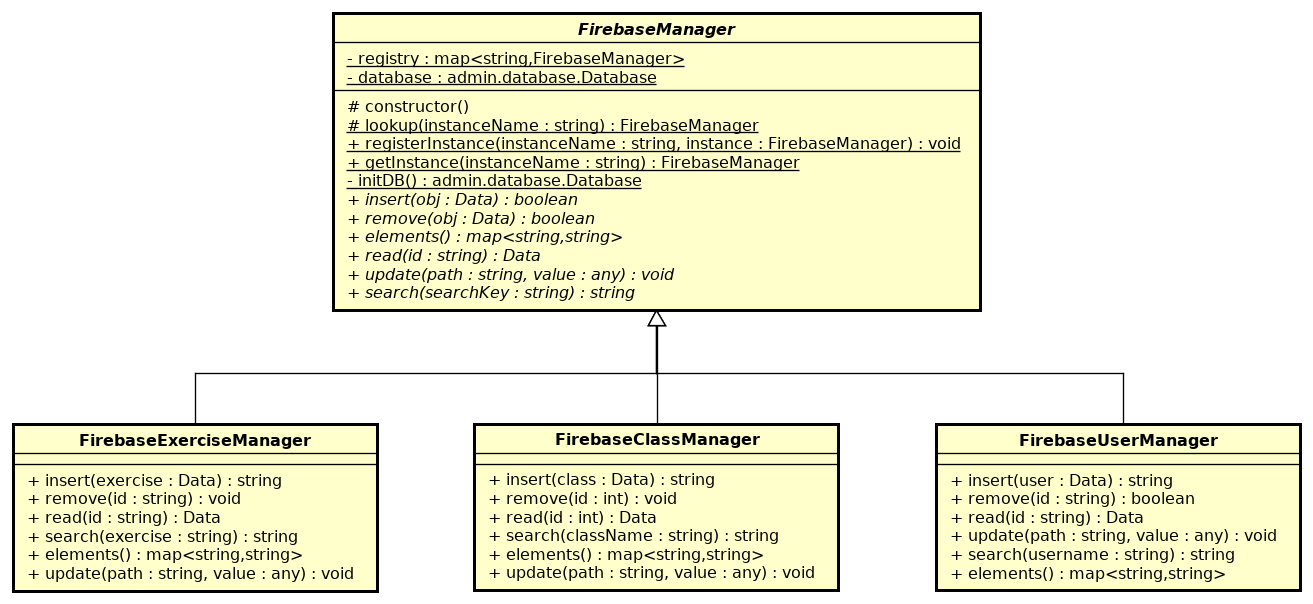
\includegraphics[scale=0.5]{images/FirebaseManager.png}
	\caption{Diagramma delle classi del package Firebase}
\end{figure}